
\documentclass[a4paper]{article}

%\VignetteIndexEntry{overlap User Manual}

\title{Overview of the \texttt{overlap} package}
\author{Mike Meredith and Martin Ridout}

\usepackage{amsmath}                  % equation numbering
\usepackage[section]{placeins}        % forces figs to be placed in current section
\usepackage[usenames,dvipsnames,svgnames]{xcolor}
\usepackage[authoryear,round]{natbib} % format for in-text citations
\usepackage[pdfstartview=]{hyperref}                 % for hypertext links
\usepackage{graphicx, Rd}
\usepackage{float}
\usepackage{Sweave}

\begin{document}
\Sconcordance{concordance:overlap.tex:overlap.Rnw:%
1 21 1 1 4 20 1 1 2 1 0 2 1 11 0 1 1 6 0 1 1 6 0 1 1 6 0 1 2 4 1 1 2 4 %
0 1 2 5 1 1 2 1 0 1 1 3 0 1 2 13 1 1 8 63 1 1 2 1 0 2 1 5 0 2 1 6 0 2 1 %
3 0 1 2 22 1 1 2 1 0 1 1 6 0 1 2 15 1 1 2 12 0 1 2 4 1 1 2 12 0 1 2 50 %
1}


\maketitle


\section{Introduction}
\label{sec:intro}

Camera traps -- cameras linked to detectors so that they fire when an animal is present -- are a major source of information on the abundance and habitat preferences of rare or shy forest animals. Modern cameras record the time of the photo, and the use of this to investigate diel~\footnote{We use ``diel" for 24-hour cycles, and reserve ``diurnal" to mean ``not nocturnal".} activity patterns was immediately recognised \citep{GriffithsVanSchaik1993}.

Initially this resulted in broad classification of taxa as diurnal, nocturnal, crepuscular, or cathemeral \citep{vanSchaikGriffiths1996}. More recently, researchers have compared activity patterns among species to see how overlapping patterns may relate to competition or predation \citep{LinkieRidout2011,Carver+2011,Ramesh+2012,Carter+2012,Kamler+2012,Ross+2013, Azevedo+2018}. % ADD  other refs?

\citet{RidoutLinkie2009} presented methods to fit kernel density functions to times of observations of animals and to estimate the coefficient of overlapping, a quantitative measure ranging from 0 (no overlap) to 1 (identical activity patterns). The code they used forms the basis of the \texttt{overlap} package.

Although motivated by the analysis of camera trap data, \texttt{overlap} could be applied to data from other sources such as data loggers, provided data collection is carried out around the clock. Nor is it limited to diel cycles: tidal cycles or seasonal cycles, such as plant flowering or fruiting or animal breeding seasons could also be investigated.


\section{Kernel density curves}
\label{sec:curve}

\subsection{Example data set}
\label{subsec:kerinci}

To demonstrate the use of the software we will use camera-trapping data from Kerinci-Seblat National Park in Sumatra, Indonesia \citep{RidoutLinkie2009}.

\begin{Schunk}
\begin{Sinput}
> library(overlap)
> data(kerinci)
> head(kerinci)
\end{Sinput}
\begin{Soutput}
  Zone   Sps  Time
1    1 tiger 0.175
2    1 tiger 0.787
3    1 tiger 0.247
4    1 tiger 0.591
5    1 tiger 0.500
6    1 tiger 0.564
\end{Soutput}
\begin{Sinput}
> table(kerinci$Zone)
\end{Sinput}
\begin{Soutput}
  1   2   3   4 
104 425 280 289 
\end{Soutput}
\begin{Sinput}
> summary(kerinci$Sps)
\end{Sinput}
\begin{Soutput}
   boar clouded  golden macaque muntjac  sambar   tapir   tiger 
     28      86     104     273     200      25     181     201 
\end{Soutput}
\begin{Sinput}
> range(kerinci$Time)
\end{Sinput}
\begin{Soutput}
[1] 0.003 0.990
\end{Soutput}
\end{Schunk}

The data provide time-of-capture data from 4 Zones within the Park for 8 species: wild pig (``\texttt{boar}''), clouded leopard, golden cat, pig-tailed macaque, common muntjac, sambar deer, tapir, and tiger.

The unit of time is the day, so values range from 0 to 1. Package \texttt{overlap} works entirely in \emph{radians}: fitting density curves uses trigonometric functions (sin, cos, tan), so this speeds up bootstraps and simulations. The conversion is straightforward:

\begin{Schunk}
\begin{Sinput}
> timeRad <- kerinci$Time * 2 * pi
\end{Sinput}
\end{Schunk}

\subsection{Fitting kernel density}
\label{subsec:density}

We will extract the data for tigers in Zone 2 (which has the most observations) and plot a kernel density curve:

\begin{Schunk}
\begin{Sinput}
> tig2 <- timeRad[kerinci$Zone == 2 & kerinci$Sps == 'tiger']
> densityPlot(tig2, rug=TRUE)
\end{Sinput}
\end{Schunk}

\begin{figure}[H]
  \centering
  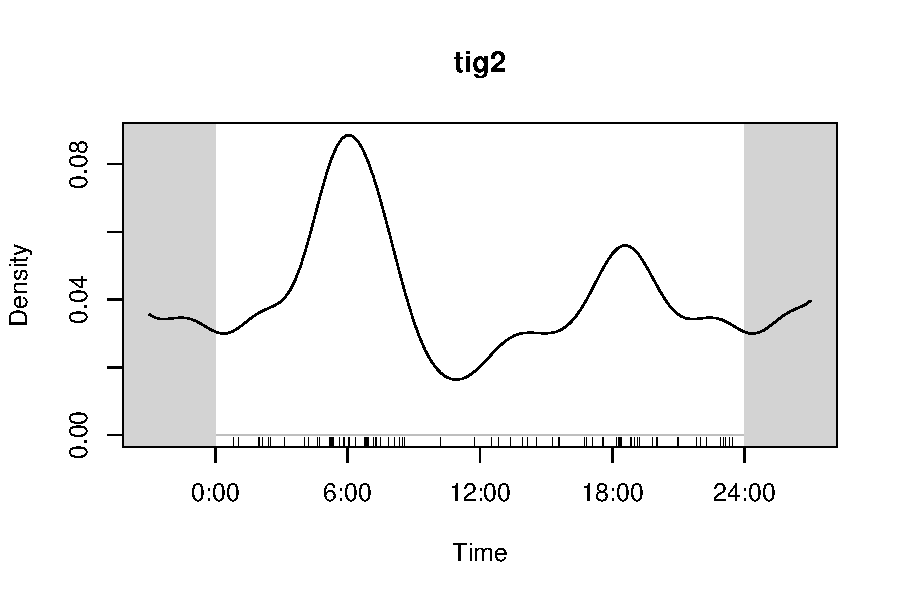
\includegraphics{overlap-singleDensityCurve}
  \caption{\it Fitted kernel density curve for tigers in Zone 3, using default smoothing parameters.}
  \label{fig:singleDensityCurve}
\end{figure}

Figure~\ref{fig:singleDensityCurve} shows the activity pattern from 21:00 to 03:00, a reminder that the density is \emph{circular}. Unlike the usual density plot that uses a Gaussian kernel, we use a von Mises kernel, corresponding to a circular distribution.

The actual data are shown at the foot of Figure~\ref{fig:singleDensityCurve} as a `rug'.

Density estimation involves smoothing the information in the data, and the degree of smoothing is controlled by the argument \code{adjust} to the \code{densityPlot} function. Increasing \code{adjust} above the default value of 1 gives a flatter curve, reducing it gives a more `spiky' curve, as shown in Figure~\ref{fig:smoothing}. The choice of \code{adjust} affects the estimate of overlap, as we discuss below.

\begin{figure}[h]
  \centering
  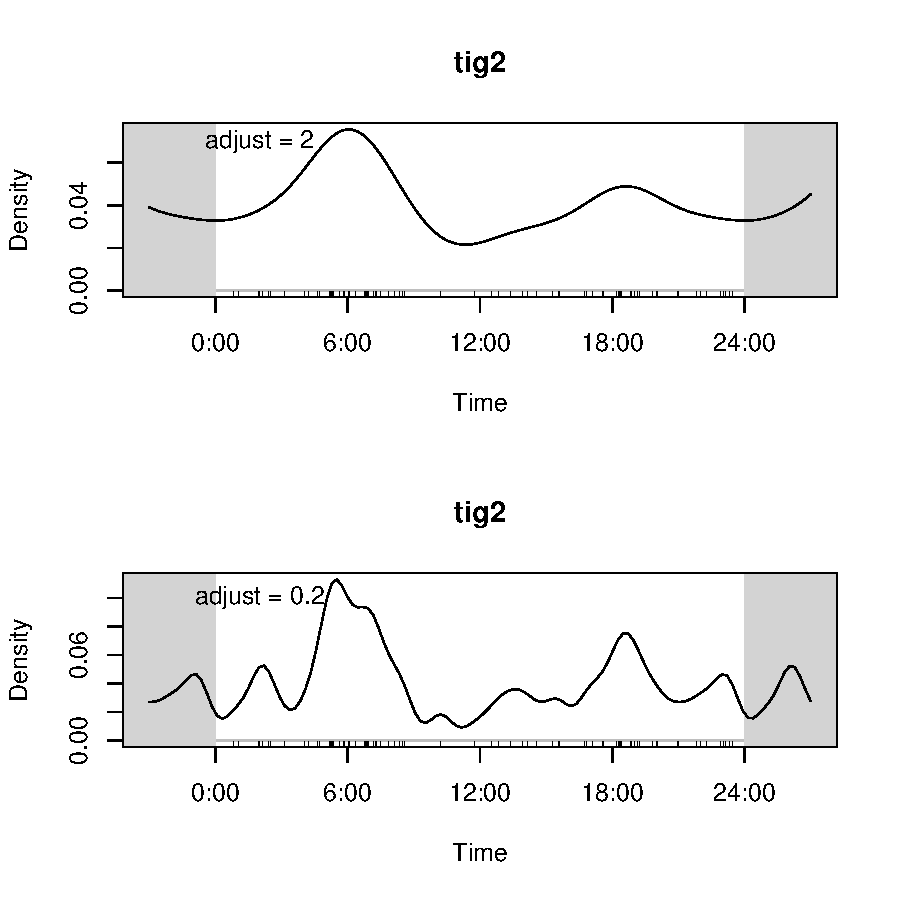
\includegraphics{overlap-smoothing}
  \caption{\it Kernel density curves fitted with different smoothing adjustments.}
  \label{fig:smoothing}
\end{figure}


\section{Quantifying overlap}
\label{sec:quantify}

Various measures of overlap have been put forward: see \citet{RidoutLinkie2009} for a review. We use the \emph{coefficient of overlapping} proposed by \citet{weitzman1970}.

\subsection{Coefficient of overlapping}
\label{subsec:coefficient}


As shown in Figure~\ref{fig:tigerMacaque2}, the coefficient of overlapping, $\Delta$, is the area lying under \emph{both} of the density curves. (Remember that the area under a density curve is, by definition, one.) Mathematically, if the two density curves are $f(x)$ and $g(x)$, this is:

\begin{equation} \label{eq:definition}
  \Delta (f, g) = \int \textrm{min} \{ f(x), g(x) \} \textrm{d}x
\end{equation}

This works if we know the true density distributions, $f(x)$ and $g(x)$; but we usually only have samples and need to estimate $\Delta$ from these.

\subsection{Estimators}
\label{subsec:estimators}

Five general nonparametric estimators of the coefficient of overlapping were proposed by \citet{SchmidSchmidt2006}. For circular distributions, the first two are equivalent and the third is unworkable \citep{RidoutLinkie2009}. We retain $\hat{\Delta}_1$,  $\hat{\Delta}_4$ and $\hat{\Delta}_5$.

The first, $\hat{\Delta}_1$, matches the definition in equation \eqref{eq:definition}, but in practice it is estimated numerically, taking a large number of values, $t_1, t_2, ..., t_T$, equally spaced between 0 and $2\pi$ ($t_i = 2\pi i/T)$ and summing:

\begin{equation} \label{eq:Dhat1}
  \hat{\Delta}_1 = \frac{1}{T} \sum_{i=1}^T \textrm{min} \{ \hat{f}(t_i), \hat{g}(t_i) \}
\end{equation}

For $\hat{\Delta}_4$ and $\hat{\Delta}_5$, we compare the densities at the observed values, $x_1,...,x_n$ for one species and $y_1, ...,y_m$ for the other:

\begin{equation} \label{eq:Dhat4}
  \hat{\Delta}_4 = \frac{1}{2} \left( \frac{1}{n} \sum_{i=1}^n \textrm{min} \left\{ 1, \frac{\hat{g}(x_i)}{\hat{f}(x_i)}\right\} + \frac{1}{m} \sum_{i=1}^m \textrm{min} \left\{ 1, \frac{\hat{f}(y_i)}{\hat{g}(y_i)}\right\} \right)
\end{equation}

\begin{equation} \label{eq:Dhat5}
  \hat{\Delta}_5 = \frac{1}{n} \sum_{i=1}^n I \left\{ \hat{f}(x_i) < \hat{g}(x_i)\right\} + \frac{1}{m} \sum_{i=1}^m I \left\{ \hat{g}(y_i) \leq \hat{f}(y_i)\right\}
\end{equation}
where $I(.)$ is 1 if the condition in the parenthesis is true, 0 otherwise.

The terms $\hat{f}(.)$ and $\hat{g}(.)$ refer to the fitted kernel density functions, and as such they are affected by the choice of the smoothing constant, \texttt{adjust}. On the basis of simulations, \citet{RidoutLinkie2009} recommend using \texttt{adjust~=~0.8} to estimate $\hat{\Delta}_1$, \texttt{adjust~=~1} for $\hat{\Delta}_4$, and \texttt{adjust~=~4} for $\hat{\Delta}_5$. (Note that \texttt{adjust} in the \texttt{overlap} functions corresponds to $1/c$ in \citet{RidoutLinkie2009}). These are the default values used in \texttt{overlap} functions.

\subsection{Choice of estimator}
\label{subsec:whichDhat}

\citet{RidoutLinkie2009} carried out simulations with a variety of scenarios where the true overlap was known, and compared the resulting estimates with the truth, calculating the root mean squared error (RMSE) for each estimator. The present authors have carried out further simulations in the same manner.

We found that the best estimator depended on the size of the \emph{smaller} of the two samples: When the smaller sample was less than 50, $\hat{\Delta}_1$ performed best, while $\hat{\Delta}_4$ was better when it was greater than 75.

In no case was $\hat{\Delta}_5$ found to be useful. It is unstable, in that small, incremental changes in the data produce discontinuous changes in the estimate, and it can give estimates greater than one.


\subsection{Examples}
\label{subsec:examples}

We will see how this works with the \texttt{kerinci} data set. We will extract the data for tigers and macaques for Zone 2, calculate the overlap with all three estimators, and plot the curves:

\begin{Schunk}
\begin{Sinput}
> tig2 <- timeRad[kerinci$Zone == 2 & kerinci$Sps == 'tiger']
> mac2 <- timeRad[kerinci$Zone == 2 & kerinci$Sps == 'macaque']
> min(length(tig2), length(mac2))
\end{Sinput}
\begin{Soutput}
[1] 83
\end{Soutput}
\begin{Sinput}
> tigmac2est <- overlapEst(tig2, mac2, type="Dhat4")
> tigmac2est
\end{Sinput}
\begin{Soutput}
    Dhat4 
0.4205464 
\end{Soutput}
\begin{Sinput}
> overlapPlot(tig2, mac2, main="Zone 2")
> legend('topright', c("Tigers", "Macaques"), lty=c(1,2), col=c(1,4), bty='n')
\end{Sinput}
\end{Schunk}
\begin{figure}[h]
  \centering
  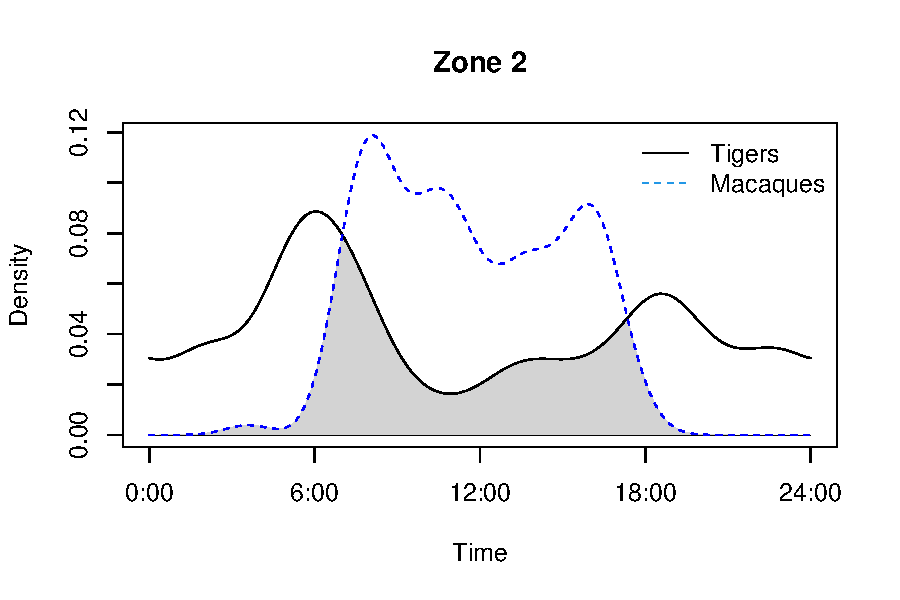
\includegraphics{overlap-tigerMacaque2}
  \caption{\it Activity curves for tigers and macaques in Zone 2. The coefficient of overlapping equals the area below both curves, shaded grey in this diagram.}
  \label{fig:tigerMacaque2}
\end{figure}

Both of these samples have more than 75 observations, so we chose to use the $\hat{\Delta}_4$ estimate, \texttt{Dhat4} in the \R{} code, giving an estimate of overlap of 0.42.

\section{Confidence intervals}
\label{sec:CIs}

To estimate confidence intervals we need to know the sampling distribution which our coefficient of overlapping is drawn from, ie, the distribution we would get if we had a very large number of independent samples from nature. The best way to investigate this is to use a bootstrap.

\subsection{The bootstrap}
\label{subsec:bootstrap}

The usual bootstrap method treats the existing sample as representative of the population, and generates a large number of new samples by randomly resampling observations with replacement from the original sample. For the case of estimating activity patterns, this may not work very well: suppose our original sample for a nocturnal species has observations ranging from 20:58 to 03:14; resampling will never yield an observation outside that range, while a fresh sample from nature may do so.

An alternative is a smoothed bootstrap. We begin by fitting a kernel density to the original data then draw random simulated observations from this distribution. Faced with original values between 20:58 and 03:14, most simulated observations would fall in the same range, but a few will fall outside.

 In the \texttt{overlap} package, we generate bootstrap samples with \texttt{bootstrap}, which has a \texttt{smooth} argument; if \texttt{smooth = TRUE} (the default), smoothed bootstrap samples are generated. For this example, we will generate just 1000 bootstrap estimates for tigers and macaques in Zone 2; for a real analysis 10,000 bootstrap samples would be better:

\begin{Schunk}
\begin{Sinput}
> tigmac2 <- bootstrap(tig2, mac2, 1000, type="Dhat4")  # takes a few seconds
> ( BSmean <- mean(tigmac2) )
\end{Sinput}
\begin{Soutput}
[1] 0.4750135
\end{Soutput}
\end{Schunk}

Note that the bootstrap mean, $\overline{BS}$, differs from $\hat{\Delta}$: 0.48 versus 0.42. The difference, $\overline{BS} - \hat{\Delta}$, is the \emph{bootstrap bias}, and we need to take this into account when calculating the confidence interval.

If the bootstrap bias were a good estimate of the original sampling bias, a better estimator of $\Delta$ would be $\tilde{\Delta} = 2\hat{\Delta} - \overline{BS}$. Our simulations show that $\tilde{\Delta}$ results in higher RMSE than the original $\hat{\Delta}$, so we do not recommend applying this correction.

\subsection{Extracting the CI}
\label{subsec:extract}

One way to estimate the confidence interval is simply to look at the appropriate percentiles of the set of bootstrap estimates (interpolating between values if necessary): for a 95\% confidence interval these would be the 2.5\% and 97.5\% percentiles. This is \texttt{perc} in the output from \texttt{overlap}'s \texttt{bootCI} function.

We noted at the end of Section~\ref{subsec:bootstrap} that, on average, the bootstrap values differ from the estimate: this is the bootstrap bias. The raw percentiles produced by \texttt{perc} need to be adjusted to account for this bias. The appropriate confidence interval is \texttt{perc} $- (\overline{BS} - \hat{\Delta})$; this is \texttt{basic0} in the \texttt{bootCI} output.

An alternative approach is to use the standard deviation of the bootstrap results, $(s_{\scriptscriptstyle BS})$, as an estimate of the spread of the sampling distribution, and then calculate the confidence interval as $\hat{\Delta} \pm z_{{\alpha}/2} s_{\scriptscriptstyle BS}$. Using $z_{0.025} = 1.96$ gives the usual 95\% confidence interval. This is \texttt{norm0} in the \texttt{bootCI} output. This procedure assumes that the sampling distribution is normal. If that's the case, \texttt{norm0} will be close to \texttt{basic0}, but if the distribution is skewed -- as it will be if $\hat{\Delta}$ is close to 0 or 1 -- \texttt{basic0} is the better estimator.

For the tiger-macaque data from Zone 2 we have the following estimates of a 95\% confidence interval:

\begin{Schunk}
\begin{Sinput}
> bootCI(tigmac2est, tigmac2)
\end{Sinput}
\begin{Soutput}
           lower     upper
norm   0.2640877 0.4680708
norm0  0.3185548 0.5225379
basic  0.2646450 0.4658881
basic0 0.3207375 0.5219806
perc   0.3752046 0.5764477
\end{Soutput}
\end{Schunk}

\texttt{bootCI} produces two further estimators: \texttt{basic} and \texttt{norm}. These are analogous to \texttt{basic0} and \texttt{norm0} but are intended for use with the bias-corrected estimator, $\tilde{\Delta}$. They match the \texttt{basic} and \texttt{norm} confidence intervals produced by \texttt{boot.ci} in package \texttt{boot}.

The coefficient of overlapping takes values in the interval [0,1]. All the confidence interval estimators except \texttt{perc} involve additive corrections which might result in values outside of this range. This can be avoided by carrying out the corrections on a logistic scale and back-transforming. This is done by \texttt{bootCIlogit}:

\begin{Schunk}
\begin{Sinput}
> bootCIlogit(tigmac2est, tigmac2)
\end{Sinput}
\begin{Soutput}
           lower     upper
norm   0.2782054 0.4683852
norm0  0.3243379 0.5231947
basic  0.2790318 0.4672696
basic0 0.3253206 0.5221690
perc   0.3752046 0.5764477
\end{Soutput}
\end{Schunk}

In this example, the CIs are well away from 0 or 1, so the difference is small (and \texttt{perc} is exactly the same as there's no correction anyway).

\subsection{Choice of CI method}
\label{subsec:whichCI}

If a series of X\% confidence intervals are calculated from independent samples from a population, we would expect X\% of them to include the true value. When running simulations we know the true value and can check the actual proportion of confidence intervals which contain the true value: this is the \emph{coverage} of the estimator. Ideally the coverage should equal the nominal confidence interval, ie, 95\% coverage for a 95\% confidence interval.

We ran a large number of simulations with different true distributions and sample sizes (see \citet{RidoutLinkie2009} for details). For each scenario, we ran both smoothed and unsmoothed bootstraps, extracted all nine 95\% confidence intervals, and checked the coverage for each.

Each estimator gave a range of coverages. We looked for a method which gave median coverage closest to the nominal 95\% and all or most values above 90\%. This was satisfied by the \texttt{basic0} estimator with smoothed bootstraps.

With small samples (smaller sample <~75) and $\Delta >~0.8$, coverage sometimes fell below 90\%, but none of the other options fared better.


\section{Summary of recommendations}
\label{sec:summary}

\begin{itemize}
  \item Use the $\hat{\Delta}_4$ estimator (\texttt{Dhat4}) if the smaller sample has more than 75 observations. Otherwise, use the $\hat{\Delta}_1$ estimator (\texttt{Dhat1}).
  \item Use a smoothed bootstrap and do at least 1000 resamples, preferably 10,000.
  \item Use the \texttt{basic0} output from \texttt{bootCI} as your confidence interval; be aware that this confidence interval will be too narrow if you have a small sample and $\Delta$ is close to 1.
\end{itemize}


\section{Caveats}
\label{sec:caveats}

\subsection{Pooling data}
\label{sec:pooling}

Pooled data give higher estimates of overlap than the original, unpooled data \citep{RidoutLinkie2009}. Suppose we find a species of bat that emerges immediately after sunset and a hawk which goes to roost just before sunset: their activity patterns do not overlap and presumably the hawk will not be feeding on the bats. But the time of sunset changes; data from December only or from June only show no overlap, but the pooled data do, and this apparent overlap is an artefact of pooling.

This is a clear-cut example. In general, differences in activity patterns across sites or time periods will be smaller, but any heterogeneity will inflate the overlap estimates from pooled data. Care is needed when comparing coefficients of overlap among study areas or periods of varying extent or degree of heterogeneity.

One way to mitigate these differences is to map "clock time" to "sun time" \citep{Nouvellet+2012}. The new function \texttt{sunTime} allows this to be done, see its help page. \citet{Azevedo+2018} used this approach for their study of puma.

\subsection{What ``activity" is observed?}
\label{sec:activity}

Camera traps set along animal trails -- as they often are -- record instances of animals moving along trails. The resulting ``activity pattern" refers to walking on trails, and overlap indicates the extent to which two species are walking on trails at the same period of the day. A browsing herbivore and the carnivore stalking it are probably both ``inactive" by this definition.

In view of this, conclusions about species interactions need to be drawn with care. In a study in Lao PDR, \citet{Kamler+2012} found that dhole and pig were active during the day and deer at night. This might suggest that dhole feed on pig rather than deer. But examination of dhole faeces showed that dhole consumed mainly deer and very little pig.


\renewcommand{\refname}{\section{References}} % Make "References" a proper, numbered section.
\bibliographystyle{jss}

\bibliography{overlap}

\end{document}
